% Options for packages loaded elsewhere
\PassOptionsToPackage{unicode}{hyperref}
\PassOptionsToPackage{hyphens}{url}
\PassOptionsToPackage{dvipsnames,svgnames,x11names}{xcolor}
%
\documentclass[
  letterpaper,
  DIV=11,
  numbers=noendperiod]{scrartcl}

\usepackage{amsmath,amssymb}
\usepackage{lmodern}
\usepackage{iftex}
\ifPDFTeX
  \usepackage[T1]{fontenc}
  \usepackage[utf8]{inputenc}
  \usepackage{textcomp} % provide euro and other symbols
\else % if luatex or xetex
  \usepackage{unicode-math}
  \defaultfontfeatures{Scale=MatchLowercase}
  \defaultfontfeatures[\rmfamily]{Ligatures=TeX,Scale=1}
\fi
% Use upquote if available, for straight quotes in verbatim environments
\IfFileExists{upquote.sty}{\usepackage{upquote}}{}
\IfFileExists{microtype.sty}{% use microtype if available
  \usepackage[]{microtype}
  \UseMicrotypeSet[protrusion]{basicmath} % disable protrusion for tt fonts
}{}
\makeatletter
\@ifundefined{KOMAClassName}{% if non-KOMA class
  \IfFileExists{parskip.sty}{%
    \usepackage{parskip}
  }{% else
    \setlength{\parindent}{0pt}
    \setlength{\parskip}{6pt plus 2pt minus 1pt}}
}{% if KOMA class
  \KOMAoptions{parskip=half}}
\makeatother
\usepackage{xcolor}
\setlength{\emergencystretch}{3em} % prevent overfull lines
\setcounter{secnumdepth}{-\maxdimen} % remove section numbering
% Make \paragraph and \subparagraph free-standing
\ifx\paragraph\undefined\else
  \let\oldparagraph\paragraph
  \renewcommand{\paragraph}[1]{\oldparagraph{#1}\mbox{}}
\fi
\ifx\subparagraph\undefined\else
  \let\oldsubparagraph\subparagraph
  \renewcommand{\subparagraph}[1]{\oldsubparagraph{#1}\mbox{}}
\fi

\usepackage{color}
\usepackage{fancyvrb}
\newcommand{\VerbBar}{|}
\newcommand{\VERB}{\Verb[commandchars=\\\{\}]}
\DefineVerbatimEnvironment{Highlighting}{Verbatim}{commandchars=\\\{\}}
% Add ',fontsize=\small' for more characters per line
\usepackage{framed}
\definecolor{shadecolor}{RGB}{241,243,245}
\newenvironment{Shaded}{\begin{snugshade}}{\end{snugshade}}
\newcommand{\AlertTok}[1]{\textcolor[rgb]{0.68,0.00,0.00}{#1}}
\newcommand{\AnnotationTok}[1]{\textcolor[rgb]{0.37,0.37,0.37}{#1}}
\newcommand{\AttributeTok}[1]{\textcolor[rgb]{0.40,0.45,0.13}{#1}}
\newcommand{\BaseNTok}[1]{\textcolor[rgb]{0.68,0.00,0.00}{#1}}
\newcommand{\BuiltInTok}[1]{\textcolor[rgb]{0.00,0.23,0.31}{#1}}
\newcommand{\CharTok}[1]{\textcolor[rgb]{0.13,0.47,0.30}{#1}}
\newcommand{\CommentTok}[1]{\textcolor[rgb]{0.37,0.37,0.37}{#1}}
\newcommand{\CommentVarTok}[1]{\textcolor[rgb]{0.37,0.37,0.37}{\textit{#1}}}
\newcommand{\ConstantTok}[1]{\textcolor[rgb]{0.56,0.35,0.01}{#1}}
\newcommand{\ControlFlowTok}[1]{\textcolor[rgb]{0.00,0.23,0.31}{#1}}
\newcommand{\DataTypeTok}[1]{\textcolor[rgb]{0.68,0.00,0.00}{#1}}
\newcommand{\DecValTok}[1]{\textcolor[rgb]{0.68,0.00,0.00}{#1}}
\newcommand{\DocumentationTok}[1]{\textcolor[rgb]{0.37,0.37,0.37}{\textit{#1}}}
\newcommand{\ErrorTok}[1]{\textcolor[rgb]{0.68,0.00,0.00}{#1}}
\newcommand{\ExtensionTok}[1]{\textcolor[rgb]{0.00,0.23,0.31}{#1}}
\newcommand{\FloatTok}[1]{\textcolor[rgb]{0.68,0.00,0.00}{#1}}
\newcommand{\FunctionTok}[1]{\textcolor[rgb]{0.28,0.35,0.67}{#1}}
\newcommand{\ImportTok}[1]{\textcolor[rgb]{0.00,0.46,0.62}{#1}}
\newcommand{\InformationTok}[1]{\textcolor[rgb]{0.37,0.37,0.37}{#1}}
\newcommand{\KeywordTok}[1]{\textcolor[rgb]{0.00,0.23,0.31}{#1}}
\newcommand{\NormalTok}[1]{\textcolor[rgb]{0.00,0.23,0.31}{#1}}
\newcommand{\OperatorTok}[1]{\textcolor[rgb]{0.37,0.37,0.37}{#1}}
\newcommand{\OtherTok}[1]{\textcolor[rgb]{0.00,0.23,0.31}{#1}}
\newcommand{\PreprocessorTok}[1]{\textcolor[rgb]{0.68,0.00,0.00}{#1}}
\newcommand{\RegionMarkerTok}[1]{\textcolor[rgb]{0.00,0.23,0.31}{#1}}
\newcommand{\SpecialCharTok}[1]{\textcolor[rgb]{0.37,0.37,0.37}{#1}}
\newcommand{\SpecialStringTok}[1]{\textcolor[rgb]{0.13,0.47,0.30}{#1}}
\newcommand{\StringTok}[1]{\textcolor[rgb]{0.13,0.47,0.30}{#1}}
\newcommand{\VariableTok}[1]{\textcolor[rgb]{0.07,0.07,0.07}{#1}}
\newcommand{\VerbatimStringTok}[1]{\textcolor[rgb]{0.13,0.47,0.30}{#1}}
\newcommand{\WarningTok}[1]{\textcolor[rgb]{0.37,0.37,0.37}{\textit{#1}}}

\providecommand{\tightlist}{%
  \setlength{\itemsep}{0pt}\setlength{\parskip}{0pt}}\usepackage{longtable,booktabs,array}
\usepackage{calc} % for calculating minipage widths
% Correct order of tables after \paragraph or \subparagraph
\usepackage{etoolbox}
\makeatletter
\patchcmd\longtable{\par}{\if@noskipsec\mbox{}\fi\par}{}{}
\makeatother
% Allow footnotes in longtable head/foot
\IfFileExists{footnotehyper.sty}{\usepackage{footnotehyper}}{\usepackage{footnote}}
\makesavenoteenv{longtable}
\usepackage{graphicx}
\makeatletter
\def\maxwidth{\ifdim\Gin@nat@width>\linewidth\linewidth\else\Gin@nat@width\fi}
\def\maxheight{\ifdim\Gin@nat@height>\textheight\textheight\else\Gin@nat@height\fi}
\makeatother
% Scale images if necessary, so that they will not overflow the page
% margins by default, and it is still possible to overwrite the defaults
% using explicit options in \includegraphics[width, height, ...]{}
\setkeys{Gin}{width=\maxwidth,height=\maxheight,keepaspectratio}
% Set default figure placement to htbp
\makeatletter
\def\fps@figure{htbp}
\makeatother

\KOMAoption{captions}{tableheading}
\makeatletter
\makeatother
\makeatletter
\makeatother
\makeatletter
\@ifpackageloaded{caption}{}{\usepackage{caption}}
\AtBeginDocument{%
\ifdefined\contentsname
  \renewcommand*\contentsname{Table of contents}
\else
  \newcommand\contentsname{Table of contents}
\fi
\ifdefined\listfigurename
  \renewcommand*\listfigurename{List of Figures}
\else
  \newcommand\listfigurename{List of Figures}
\fi
\ifdefined\listtablename
  \renewcommand*\listtablename{List of Tables}
\else
  \newcommand\listtablename{List of Tables}
\fi
\ifdefined\figurename
  \renewcommand*\figurename{Figure}
\else
  \newcommand\figurename{Figure}
\fi
\ifdefined\tablename
  \renewcommand*\tablename{Table}
\else
  \newcommand\tablename{Table}
\fi
}
\@ifpackageloaded{float}{}{\usepackage{float}}
\floatstyle{ruled}
\@ifundefined{c@chapter}{\newfloat{codelisting}{h}{lop}}{\newfloat{codelisting}{h}{lop}[chapter]}
\floatname{codelisting}{Listing}
\newcommand*\listoflistings{\listof{codelisting}{List of Listings}}
\makeatother
\makeatletter
\@ifpackageloaded{caption}{}{\usepackage{caption}}
\@ifpackageloaded{subcaption}{}{\usepackage{subcaption}}
\makeatother
\makeatletter
\@ifpackageloaded{tcolorbox}{}{\usepackage[many]{tcolorbox}}
\makeatother
\makeatletter
\@ifundefined{shadecolor}{\definecolor{shadecolor}{rgb}{.97, .97, .97}}
\makeatother
\makeatletter
\makeatother
\ifLuaTeX
  \usepackage{selnolig}  % disable illegal ligatures
\fi
\IfFileExists{bookmark.sty}{\usepackage{bookmark}}{\usepackage{hyperref}}
\IfFileExists{xurl.sty}{\usepackage{xurl}}{} % add URL line breaks if available
\urlstyle{same} % disable monospaced font for URLs
\hypersetup{
  pdftitle={Class13},
  pdfauthor={Max Strul},
  colorlinks=true,
  linkcolor={blue},
  filecolor={Maroon},
  citecolor={Blue},
  urlcolor={Blue},
  pdfcreator={LaTeX via pandoc}}

\title{Class13}
\author{Max Strul}
\date{11-9-2022}

\begin{document}
\maketitle
\ifdefined\Shaded\renewenvironment{Shaded}{\begin{tcolorbox}[breakable, borderline west={3pt}{0pt}{shadecolor}, interior hidden, boxrule=0pt, enhanced, sharp corners, frame hidden]}{\end{tcolorbox}}\fi

\renewcommand*\contentsname{Table of contents}
{
\hypersetup{linkcolor=}
\setcounter{tocdepth}{3}
\tableofcontents
}
\hypertarget{outline-for-setting-up-rnaseq-data}{%
\section{Outline for setting up RNAseq
data}\label{outline-for-setting-up-rnaseq-data}}

\begin{itemize}
\tightlist
\item
  1.) Read input files,

  \begin{itemize}
  \tightlist
  \item
    a.) countdata
  \item
    b.) coldata
  \end{itemize}
\item
  2.) Check and fix

  \begin{itemize}
  \tightlist
  \item
    a.) remove zero count genes across all
  \end{itemize}
\item
  3.)DESEQ

  \begin{itemize}
  \tightlist
  \item
    a.) plot of Log2fc vs -log(p-value)
  \item
    b.)write csv of results
  \end{itemize}
\item
  4.) Annotation
\item
  5.) Pathway analysis
\end{itemize}

Getting our data ready:

\begin{Shaded}
\begin{Highlighting}[]
\FunctionTok{library}\NormalTok{(}\StringTok{"DESeq2"}\NormalTok{)}
\end{Highlighting}
\end{Shaded}

\begin{verbatim}
Loading required package: S4Vectors
\end{verbatim}

\begin{verbatim}
Loading required package: stats4
\end{verbatim}

\begin{verbatim}
Loading required package: BiocGenerics
\end{verbatim}

\begin{verbatim}

Attaching package: 'BiocGenerics'
\end{verbatim}

\begin{verbatim}
The following objects are masked from 'package:stats':

    IQR, mad, sd, var, xtabs
\end{verbatim}

\begin{verbatim}
The following objects are masked from 'package:base':

    anyDuplicated, append, as.data.frame, basename, cbind, colnames,
    dirname, do.call, duplicated, eval, evalq, Filter, Find, get, grep,
    grepl, intersect, is.unsorted, lapply, Map, mapply, match, mget,
    order, paste, pmax, pmax.int, pmin, pmin.int, Position, rank,
    rbind, Reduce, rownames, sapply, setdiff, sort, table, tapply,
    union, unique, unsplit, which.max, which.min
\end{verbatim}

\begin{verbatim}

Attaching package: 'S4Vectors'
\end{verbatim}

\begin{verbatim}
The following objects are masked from 'package:base':

    expand.grid, I, unname
\end{verbatim}

\begin{verbatim}
Loading required package: IRanges
\end{verbatim}

\begin{verbatim}
Loading required package: GenomicRanges
\end{verbatim}

\begin{verbatim}
Loading required package: GenomeInfoDb
\end{verbatim}

\begin{verbatim}
Loading required package: SummarizedExperiment
\end{verbatim}

\begin{verbatim}
Loading required package: MatrixGenerics
\end{verbatim}

\begin{verbatim}
Loading required package: matrixStats
\end{verbatim}

\begin{verbatim}

Attaching package: 'MatrixGenerics'
\end{verbatim}

\begin{verbatim}
The following objects are masked from 'package:matrixStats':

    colAlls, colAnyNAs, colAnys, colAvgsPerRowSet, colCollapse,
    colCounts, colCummaxs, colCummins, colCumprods, colCumsums,
    colDiffs, colIQRDiffs, colIQRs, colLogSumExps, colMadDiffs,
    colMads, colMaxs, colMeans2, colMedians, colMins, colOrderStats,
    colProds, colQuantiles, colRanges, colRanks, colSdDiffs, colSds,
    colSums2, colTabulates, colVarDiffs, colVars, colWeightedMads,
    colWeightedMeans, colWeightedMedians, colWeightedSds,
    colWeightedVars, rowAlls, rowAnyNAs, rowAnys, rowAvgsPerColSet,
    rowCollapse, rowCounts, rowCummaxs, rowCummins, rowCumprods,
    rowCumsums, rowDiffs, rowIQRDiffs, rowIQRs, rowLogSumExps,
    rowMadDiffs, rowMads, rowMaxs, rowMeans2, rowMedians, rowMins,
    rowOrderStats, rowProds, rowQuantiles, rowRanges, rowRanks,
    rowSdDiffs, rowSds, rowSums2, rowTabulates, rowVarDiffs, rowVars,
    rowWeightedMads, rowWeightedMeans, rowWeightedMedians,
    rowWeightedSds, rowWeightedVars
\end{verbatim}

\begin{verbatim}
Loading required package: Biobase
\end{verbatim}

\begin{verbatim}
Welcome to Bioconductor

    Vignettes contain introductory material; view with
    'browseVignettes()'. To cite Bioconductor, see
    'citation("Biobase")', and for packages 'citation("pkgname")'.
\end{verbatim}

\begin{verbatim}

Attaching package: 'Biobase'
\end{verbatim}

\begin{verbatim}
The following object is masked from 'package:MatrixGenerics':

    rowMedians
\end{verbatim}

\begin{verbatim}
The following objects are masked from 'package:matrixStats':

    anyMissing, rowMedians
\end{verbatim}

\hypertarget{readinputfiles}{%
\section{ReadInputFiles}\label{readinputfiles}}

\begin{Shaded}
\begin{Highlighting}[]
\NormalTok{metaFile }\OtherTok{\textless{}{-}} \StringTok{"GSE37704\_metadata.csv"}
\NormalTok{countFile }\OtherTok{\textless{}{-}} \StringTok{"GSE37704\_featurecounts.csv"}
\NormalTok{colData }\OtherTok{=} \FunctionTok{read.csv}\NormalTok{(metaFile, }\AttributeTok{row.names =} \DecValTok{1}\NormalTok{)}
\FunctionTok{head}\NormalTok{(colData)}
\end{Highlighting}
\end{Shaded}

\begin{verbatim}
              condition
SRR493366 control_sirna
SRR493367 control_sirna
SRR493368 control_sirna
SRR493369      hoxa1_kd
SRR493370      hoxa1_kd
SRR493371      hoxa1_kd
\end{verbatim}

\begin{Shaded}
\begin{Highlighting}[]
\NormalTok{countdata }\OtherTok{=} \FunctionTok{read.csv}\NormalTok{(countFile, }\AttributeTok{row.names=}\DecValTok{1}\NormalTok{)}
\FunctionTok{head}\NormalTok{(countdata)}
\end{Highlighting}
\end{Shaded}

\begin{verbatim}
                length SRR493366 SRR493367 SRR493368 SRR493369 SRR493370
ENSG00000186092    918         0         0         0         0         0
ENSG00000279928    718         0         0         0         0         0
ENSG00000279457   1982        23        28        29        29        28
ENSG00000278566    939         0         0         0         0         0
ENSG00000273547    939         0         0         0         0         0
ENSG00000187634   3214       124       123       205       207       212
                SRR493371
ENSG00000186092         0
ENSG00000279928         0
ENSG00000279457        46
ENSG00000278566         0
ENSG00000273547         0
ENSG00000187634       258
\end{verbatim}

\begin{Shaded}
\begin{Highlighting}[]
\FunctionTok{length}\NormalTok{(countdata}\SpecialCharTok{$}\NormalTok{SRR493366)}
\end{Highlighting}
\end{Shaded}

\begin{verbatim}
[1] 19808
\end{verbatim}

\begin{Shaded}
\begin{Highlighting}[]
\NormalTok{countData }\OtherTok{\textless{}{-}} \FunctionTok{as.matrix}\NormalTok{(countdata[,}\SpecialCharTok{{-}}\DecValTok{1}\NormalTok{])}
\FunctionTok{head}\NormalTok{(countData)}
\end{Highlighting}
\end{Shaded}

\begin{verbatim}
                SRR493366 SRR493367 SRR493368 SRR493369 SRR493370 SRR493371
ENSG00000186092         0         0         0         0         0         0
ENSG00000279928         0         0         0         0         0         0
ENSG00000279457        23        28        29        29        28        46
ENSG00000278566         0         0         0         0         0         0
ENSG00000273547         0         0         0         0         0         0
ENSG00000187634       124       123       205       207       212       258
\end{verbatim}

Whats the point of having colnames if our data frame can initially just
have the experimental conditions?

\hypertarget{check-and-fix}{%
\section{Check and Fix}\label{check-and-fix}}

\begin{Shaded}
\begin{Highlighting}[]
\NormalTok{counts }\OtherTok{\textless{}{-}}\NormalTok{ countData[}\FunctionTok{rowSums}\NormalTok{(countData)}\SpecialCharTok{!=}\DecValTok{0}\NormalTok{,]}
\FunctionTok{head}\NormalTok{(counts)}
\end{Highlighting}
\end{Shaded}

\begin{verbatim}
                SRR493366 SRR493367 SRR493368 SRR493369 SRR493370 SRR493371
ENSG00000279457        23        28        29        29        28        46
ENSG00000187634       124       123       205       207       212       258
ENSG00000188976      1637      1831      2383      1226      1326      1504
ENSG00000187961       120       153       180       236       255       357
ENSG00000187583        24        48        65        44        48        64
ENSG00000187642         4         9        16        14        16        16
\end{verbatim}

\begin{Shaded}
\begin{Highlighting}[]
\FunctionTok{length}\NormalTok{(counts[,}\DecValTok{1}\NormalTok{])}
\end{Highlighting}
\end{Shaded}

\begin{verbatim}
[1] 15975
\end{verbatim}

number of genes removed

\begin{Shaded}
\begin{Highlighting}[]
\DecValTok{19808{-}15975}
\end{Highlighting}
\end{Shaded}

\begin{verbatim}
[1] 3833
\end{verbatim}

\hypertarget{qc-wth-pca}{%
\section{QC wth PCA}\label{qc-wth-pca}}

the \texttt{prcomp()} function in base R can do some ``QC''. It will
check if there are unique groups differentially separated based on the
read counts

For prcomps we will ensure that we scale our data

\begin{Shaded}
\begin{Highlighting}[]
\NormalTok{pca }\OtherTok{\textless{}{-}} \FunctionTok{prcomp}\NormalTok{(}\FunctionTok{t}\NormalTok{(counts),}\AttributeTok{scale=}\ConstantTok{TRUE}\NormalTok{)}
\FunctionTok{summary}\NormalTok{(pca)}
\end{Highlighting}
\end{Shaded}

\begin{verbatim}
Importance of components:
                           PC1     PC2      PC3      PC4      PC5       PC6
Standard deviation     87.7211 73.3196 32.89604 31.15094 29.18417 6.648e-13
Proportion of Variance  0.4817  0.3365  0.06774  0.06074  0.05332 0.000e+00
Cumulative Proportion   0.4817  0.8182  0.88594  0.94668  1.00000 1.000e+00
\end{verbatim}

Here we see the frist two PCS cover about 82 \% of variance

\begin{Shaded}
\begin{Highlighting}[]
\FunctionTok{plot}\NormalTok{(pca}\SpecialCharTok{$}\NormalTok{x[,}\DecValTok{1}\NormalTok{],pca}\SpecialCharTok{$}\NormalTok{x[,}\DecValTok{2}\NormalTok{],}\AttributeTok{col=}\FunctionTok{factor}\NormalTok{(colData}\SpecialCharTok{$}\NormalTok{condition))}
\end{Highlighting}
\end{Shaded}

\begin{figure}[H]

{\centering 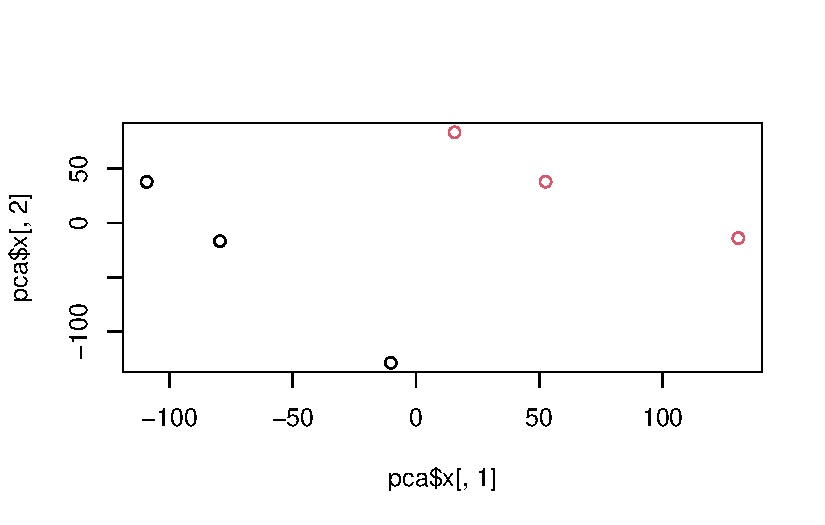
\includegraphics{class_13_files/figure-pdf/unnamed-chunk-7-1.pdf}

}

\end{figure}

Why does PCA give QC? Cant a PCA be used to find variance unrelated to
the different groups regardless of any other data? its job is to find
some way to manipulate the data to find differences in the groups that
allow us to separate it out? \# DESeq

\begin{Shaded}
\begin{Highlighting}[]
\NormalTok{dds }\OtherTok{=} \FunctionTok{DESeqDataSetFromMatrix}\NormalTok{(}\AttributeTok{countData=}\NormalTok{counts,}
                             \AttributeTok{colData =}\NormalTok{ colData,}
                             \AttributeTok{design=}\SpecialCharTok{\textasciitilde{}}\NormalTok{condition)}
\end{Highlighting}
\end{Shaded}

\begin{verbatim}
Warning in DESeqDataSet(se, design = design, ignoreRank): some variables in
design formula are characters, converting to factors
\end{verbatim}

\begin{Shaded}
\begin{Highlighting}[]
\NormalTok{dds }\OtherTok{=} \FunctionTok{DESeq}\NormalTok{(dds)}
\end{Highlighting}
\end{Shaded}

\begin{verbatim}
estimating size factors
\end{verbatim}

\begin{verbatim}
estimating dispersions
\end{verbatim}

\begin{verbatim}
gene-wise dispersion estimates
\end{verbatim}

\begin{verbatim}
mean-dispersion relationship
\end{verbatim}

\begin{verbatim}
final dispersion estimates
\end{verbatim}

\begin{verbatim}
fitting model and testing
\end{verbatim}

\begin{Shaded}
\begin{Highlighting}[]
\NormalTok{dds}
\end{Highlighting}
\end{Shaded}

\begin{verbatim}
class: DESeqDataSet 
dim: 15975 6 
metadata(1): version
assays(4): counts mu H cooks
rownames(15975): ENSG00000279457 ENSG00000187634 ... ENSG00000276345
  ENSG00000271254
rowData names(22): baseMean baseVar ... deviance maxCooks
colnames(6): SRR493366 SRR493367 ... SRR493370 SRR493371
colData names(2): condition sizeFactor
\end{verbatim}

\begin{Shaded}
\begin{Highlighting}[]
\NormalTok{res }\OtherTok{=} \FunctionTok{results}\NormalTok{(dds)}

\FunctionTok{summary}\NormalTok{(res)}
\end{Highlighting}
\end{Shaded}

\begin{verbatim}

out of 15975 with nonzero total read count
adjusted p-value < 0.1
LFC > 0 (up)       : 4349, 27%
LFC < 0 (down)     : 4396, 28%
outliers [1]       : 0, 0%
low counts [2]     : 1237, 7.7%
(mean count < 0)
[1] see 'cooksCutoff' argument of ?results
[2] see 'independentFiltering' argument of ?results
\end{verbatim}

\begin{Shaded}
\begin{Highlighting}[]
\FunctionTok{plot}\NormalTok{(res}\SpecialCharTok{$}\NormalTok{log2FoldChange,}\SpecialCharTok{{-}}\FunctionTok{log}\NormalTok{(res}\SpecialCharTok{$}\NormalTok{padj))}
\end{Highlighting}
\end{Shaded}

\begin{figure}[H]

{\centering 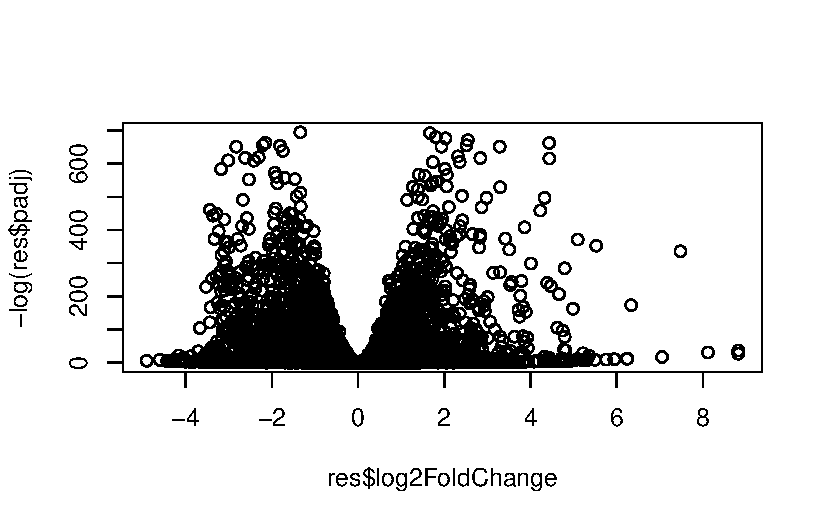
\includegraphics{class_13_files/figure-pdf/unnamed-chunk-10-1.pdf}

}

\end{figure}

\begin{Shaded}
\begin{Highlighting}[]
\NormalTok{mycols }\OtherTok{\textless{}{-}} \FunctionTok{rep}\NormalTok{(}\StringTok{"gray"}\NormalTok{,}\FunctionTok{nrow}\NormalTok{(res))}

\NormalTok{mycols[}\FunctionTok{abs}\NormalTok{(res}\SpecialCharTok{$}\NormalTok{log2FoldChange)}\SpecialCharTok{\textgreater{}}\DecValTok{2}\NormalTok{] }\OtherTok{\textless{}{-}} \StringTok{"red"}
\NormalTok{inds }\OtherTok{\textless{}{-}}\NormalTok{ (res}\SpecialCharTok{$}\NormalTok{padj}\SpecialCharTok{\textless{}}\FloatTok{0.05} \SpecialCharTok{\&} \FunctionTok{abs}\NormalTok{(res}\SpecialCharTok{$}\NormalTok{log2FoldChange)}\SpecialCharTok{\textgreater{}}\DecValTok{2}\NormalTok{)}
\NormalTok{mycols[inds] }\OtherTok{\textless{}{-}} \StringTok{"blue"}
\FunctionTok{plot}\NormalTok{(res}\SpecialCharTok{$}\NormalTok{log2FoldChange, }\SpecialCharTok{{-}} \FunctionTok{log}\NormalTok{(res}\SpecialCharTok{$}\NormalTok{padj),}\AttributeTok{col=}\NormalTok{mycols, }\AttributeTok{xlab=}\StringTok{"Log2(FoldChange)"}\NormalTok{, }\AttributeTok{ylab=}\StringTok{"{-}Log(P{-}value)"}\NormalTok{)}
\end{Highlighting}
\end{Shaded}

\begin{figure}[H]

{\centering 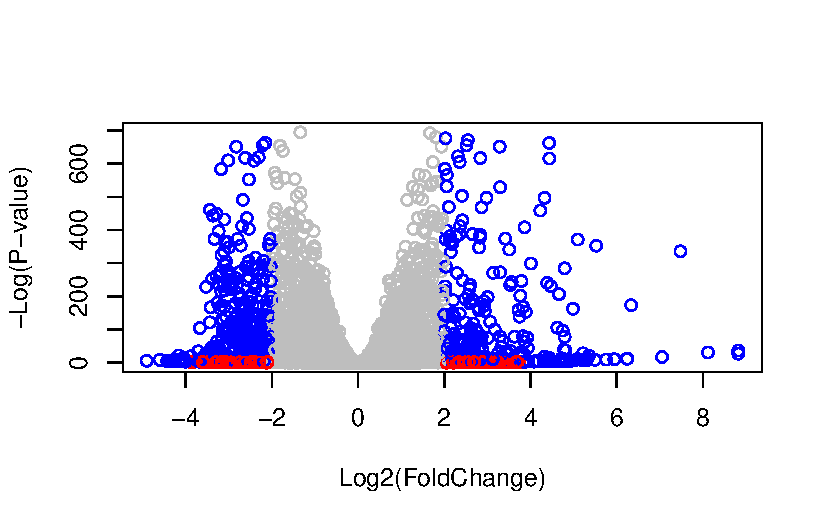
\includegraphics{class_13_files/figure-pdf/unnamed-chunk-11-1.pdf}

}

\end{figure}

\hypertarget{annotation}{%
\section{Annotation}\label{annotation}}

\begin{Shaded}
\begin{Highlighting}[]
\FunctionTok{library}\NormalTok{(}\StringTok{"AnnotationDbi"}\NormalTok{)}
\FunctionTok{library}\NormalTok{(}\StringTok{"org.Hs.eg.db"}\NormalTok{)}
\end{Highlighting}
\end{Shaded}

\begin{verbatim}
\end{verbatim}

\begin{Shaded}
\begin{Highlighting}[]
\FunctionTok{columns}\NormalTok{(org.Hs.eg.db)}
\end{Highlighting}
\end{Shaded}

\begin{verbatim}
 [1] "ACCNUM"       "ALIAS"        "ENSEMBL"      "ENSEMBLPROT"  "ENSEMBLTRANS"
 [6] "ENTREZID"     "ENZYME"       "EVIDENCE"     "EVIDENCEALL"  "GENENAME"    
[11] "GENETYPE"     "GO"           "GOALL"        "IPI"          "MAP"         
[16] "OMIM"         "ONTOLOGY"     "ONTOLOGYALL"  "PATH"         "PFAM"        
[21] "PMID"         "PROSITE"      "REFSEQ"       "SYMBOL"       "UCSCKG"      
[26] "UNIPROT"     
\end{verbatim}

\begin{Shaded}
\begin{Highlighting}[]
\NormalTok{res}\SpecialCharTok{$}\NormalTok{symbol }\OtherTok{=} \FunctionTok{mapIds}\NormalTok{(org.Hs.eg.db,}
                    \AttributeTok{keys=}\FunctionTok{rownames}\NormalTok{(counts),}
                    \AttributeTok{keytype=}\StringTok{"ENSEMBL"}\NormalTok{,}
                    \AttributeTok{column=}\StringTok{"SYMBOL"}\NormalTok{)}
\end{Highlighting}
\end{Shaded}

\begin{verbatim}
'select()' returned 1:many mapping between keys and columns
\end{verbatim}

\begin{Shaded}
\begin{Highlighting}[]
\NormalTok{res}\SpecialCharTok{$}\NormalTok{entrez }\OtherTok{=} \FunctionTok{mapIds}\NormalTok{(org.Hs.eg.db,}
                    \AttributeTok{keys=}\FunctionTok{rownames}\NormalTok{(counts),}
                    \AttributeTok{keytype=}\StringTok{"ENSEMBL"}\NormalTok{,}
                    \AttributeTok{column=}\StringTok{"ENTREZID"}\NormalTok{)}
\end{Highlighting}
\end{Shaded}

\begin{verbatim}
'select()' returned 1:many mapping between keys and columns
\end{verbatim}

\begin{Shaded}
\begin{Highlighting}[]
\NormalTok{res}\SpecialCharTok{$}\NormalTok{name }\OtherTok{=} \FunctionTok{mapIds}\NormalTok{(org.Hs.eg.db,}
                  \AttributeTok{keys=}\FunctionTok{rownames}\NormalTok{(counts),}
                  \AttributeTok{keytype=}\StringTok{"ENSEMBL"}\NormalTok{,}
                  \AttributeTok{column=}\StringTok{"GENENAME"}\NormalTok{)}
\end{Highlighting}
\end{Shaded}

\begin{verbatim}
'select()' returned 1:many mapping between keys and columns
\end{verbatim}

\begin{Shaded}
\begin{Highlighting}[]
\FunctionTok{head}\NormalTok{(res)}
\end{Highlighting}
\end{Shaded}

\begin{verbatim}
log2 fold change (MLE): condition hoxa1 kd vs control sirna 
Wald test p-value: condition hoxa1 kd vs control sirna 
DataFrame with 6 rows and 9 columns
                 baseMean log2FoldChange     lfcSE       stat      pvalue
                <numeric>      <numeric> <numeric>  <numeric>   <numeric>
ENSG00000279457   29.9136      0.1792571 0.3248216   0.551863 5.81042e-01
ENSG00000187634  183.2296      0.4264571 0.1402658   3.040350 2.36304e-03
ENSG00000188976 1651.1881     -0.6927205 0.0548465 -12.630158 1.43990e-36
ENSG00000187961  209.6379      0.7297556 0.1318599   5.534326 3.12428e-08
ENSG00000187583   47.2551      0.0405765 0.2718928   0.149237 8.81366e-01
ENSG00000187642   11.9798      0.5428105 0.5215598   1.040744 2.97994e-01
                       padj      symbol      entrez                   name
                  <numeric> <character> <character>            <character>
ENSG00000279457 6.86555e-01          NA          NA                     NA
ENSG00000187634 5.15718e-03      SAMD11      148398 sterile alpha motif ..
ENSG00000188976 1.76549e-35       NOC2L       26155 NOC2 like nucleolar ..
ENSG00000187961 1.13413e-07      KLHL17      339451 kelch like family me..
ENSG00000187583 9.19031e-01     PLEKHN1       84069 pleckstrin homology ..
ENSG00000187642 4.03379e-01       PERM1       84808 PPARGC1 and ESRR ind..
\end{verbatim}

loading up pathway analysis

\hypertarget{pathway-analysis}{%
\section{Pathway Analysis}\label{pathway-analysis}}

\begin{Shaded}
\begin{Highlighting}[]
\FunctionTok{library}\NormalTok{(}\StringTok{"pathview"}\NormalTok{)}
\end{Highlighting}
\end{Shaded}

\begin{verbatim}
##############################################################################
Pathview is an open source software package distributed under GNU General
Public License version 3 (GPLv3). Details of GPLv3 is available at
http://www.gnu.org/licenses/gpl-3.0.html. Particullary, users are required to
formally cite the original Pathview paper (not just mention it) in publications
or products. For details, do citation("pathview") within R.

The pathview downloads and uses KEGG data. Non-academic uses may require a KEGG
license agreement (details at http://www.kegg.jp/kegg/legal.html).
##############################################################################
\end{verbatim}

\begin{Shaded}
\begin{Highlighting}[]
\FunctionTok{library}\NormalTok{(}\StringTok{"gage"}\NormalTok{)}
\end{Highlighting}
\end{Shaded}

\begin{verbatim}
\end{verbatim}

\begin{Shaded}
\begin{Highlighting}[]
\FunctionTok{library}\NormalTok{(}\StringTok{"gageData"}\NormalTok{)}
\FunctionTok{data}\NormalTok{(}\StringTok{"kegg.sets.hs"}\NormalTok{)}
\FunctionTok{data}\NormalTok{(}\StringTok{"sigmet.idx.hs"}\NormalTok{)}
\NormalTok{kegg.sets.hs}\OtherTok{=}\NormalTok{kegg.sets.hs[sigmet.idx.hs]}
\NormalTok{foldchanges}\OtherTok{=}\NormalTok{res}\SpecialCharTok{$}\NormalTok{log2FoldChange}
\FunctionTok{names}\NormalTok{(foldchanges)}\OtherTok{=}\NormalTok{res}\SpecialCharTok{$}\NormalTok{entrez}
\FunctionTok{head}\NormalTok{(foldchanges)}
\end{Highlighting}
\end{Shaded}

\begin{verbatim}
       <NA>      148398       26155      339451       84069       84808 
 0.17925708  0.42645712 -0.69272046  0.72975561  0.04057653  0.54281049 
\end{verbatim}

gage pathway analysis

\begin{Shaded}
\begin{Highlighting}[]
\NormalTok{keggres }\OtherTok{=} \FunctionTok{gage}\NormalTok{(foldchanges,}\AttributeTok{gsets=}\NormalTok{kegg.sets.hs)}

\FunctionTok{attributes}\NormalTok{(keggres)}
\end{Highlighting}
\end{Shaded}

\begin{verbatim}
$names
[1] "greater" "less"    "stats"  
\end{verbatim}

\begin{Shaded}
\begin{Highlighting}[]
\FunctionTok{head}\NormalTok{(keggres}\SpecialCharTok{$}\NormalTok{less)}
\end{Highlighting}
\end{Shaded}

\begin{verbatim}
                                         p.geomean stat.mean        p.val
hsa04110 Cell cycle                   8.995727e-06 -4.378644 8.995727e-06
hsa03030 DNA replication              9.424076e-05 -3.951803 9.424076e-05
hsa03013 RNA transport                1.246882e-03 -3.059466 1.246882e-03
hsa03440 Homologous recombination     3.066756e-03 -2.852899 3.066756e-03
hsa04114 Oocyte meiosis               3.784520e-03 -2.698128 3.784520e-03
hsa00010 Glycolysis / Gluconeogenesis 8.961413e-03 -2.405398 8.961413e-03
                                            q.val set.size         exp1
hsa04110 Cell cycle                   0.001448312      121 8.995727e-06
hsa03030 DNA replication              0.007586381       36 9.424076e-05
hsa03013 RNA transport                0.066915974      144 1.246882e-03
hsa03440 Homologous recombination     0.121861535       28 3.066756e-03
hsa04114 Oocyte meiosis               0.121861535      102 3.784520e-03
hsa00010 Glycolysis / Gluconeogenesis 0.212222694       53 8.961413e-03
\end{verbatim}

\begin{Shaded}
\begin{Highlighting}[]
\FunctionTok{head}\NormalTok{(keggres}\SpecialCharTok{$}\NormalTok{greater)}
\end{Highlighting}
\end{Shaded}

\begin{verbatim}
                                        p.geomean stat.mean       p.val
hsa04640 Hematopoietic cell lineage   0.002822776  2.833362 0.002822776
hsa04630 Jak-STAT signaling pathway   0.005202070  2.585673 0.005202070
hsa00140 Steroid hormone biosynthesis 0.007255099  2.526744 0.007255099
hsa04142 Lysosome                     0.010107392  2.338364 0.010107392
hsa04330 Notch signaling pathway      0.018747253  2.111725 0.018747253
hsa04916 Melanogenesis                0.019399766  2.081927 0.019399766
                                          q.val set.size        exp1
hsa04640 Hematopoietic cell lineage   0.3893570       55 0.002822776
hsa04630 Jak-STAT signaling pathway   0.3893570      109 0.005202070
hsa00140 Steroid hormone biosynthesis 0.3893570       31 0.007255099
hsa04142 Lysosome                     0.4068225      118 0.010107392
hsa04330 Notch signaling pathway      0.4391731       46 0.018747253
hsa04916 Melanogenesis                0.4391731       90 0.019399766
\end{verbatim}

Can I create my own gsets? a list of known symbols or entrez iDS? and
see what is less or greater?

pathview function

\begin{Shaded}
\begin{Highlighting}[]
\FunctionTok{pathview}\NormalTok{(}\AttributeTok{gene.data=}\NormalTok{foldchanges,}\AttributeTok{pathway.id=}\StringTok{"hsa04110"}\NormalTok{)}
\end{Highlighting}
\end{Shaded}

\begin{verbatim}
'select()' returned 1:1 mapping between keys and columns
\end{verbatim}

\begin{verbatim}
Info: Working in directory /Users/maxstrul/Desktop/BGGN213/Rfiles/Class13/Class13
\end{verbatim}

\begin{verbatim}
Info: Writing image file hsa04110.pathview.png
\end{verbatim}

\begin{Shaded}
\begin{Highlighting}[]
\FunctionTok{pathview}\NormalTok{(}\AttributeTok{gene.data=}\NormalTok{foldchanges,}\AttributeTok{pathway.id=}\StringTok{"hsa00140"}\NormalTok{)}
\end{Highlighting}
\end{Shaded}

\begin{verbatim}
'select()' returned 1:1 mapping between keys and columns
\end{verbatim}

\begin{verbatim}
Info: Working in directory /Users/maxstrul/Desktop/BGGN213/Rfiles/Class13/Class13
\end{verbatim}

\begin{verbatim}
Info: Writing image file hsa00140.pathview.png
\end{verbatim}

\begin{Shaded}
\begin{Highlighting}[]
\FunctionTok{data}\NormalTok{(go.sets.hs)}
\FunctionTok{data}\NormalTok{(go.subs.hs)}
\NormalTok{gobpsets }\OtherTok{=}\NormalTok{ go.sets.hs[go.subs.hs}\SpecialCharTok{$}\NormalTok{BP]}
\CommentTok{\#gobpsets = go.sets.hs\#[go.subs.hs$BP]}
\NormalTok{gobpres }\OtherTok{=} \FunctionTok{gage}\NormalTok{(foldchanges,}\AttributeTok{gsets=}\NormalTok{gobpsets, }\AttributeTok{same.dir=}\ConstantTok{TRUE}\NormalTok{)}
\FunctionTok{lapply}\NormalTok{(gobpres,head)}
\end{Highlighting}
\end{Shaded}

\begin{verbatim}
$greater
                                             p.geomean stat.mean        p.val
GO:0007156 homophilic cell adhesion       8.519724e-05  3.824205 8.519724e-05
GO:0002009 morphogenesis of an epithelium 1.396681e-04  3.653886 1.396681e-04
GO:0048729 tissue morphogenesis           1.432451e-04  3.643242 1.432451e-04
GO:0007610 behavior                       2.195494e-04  3.530241 2.195494e-04
GO:0060562 epithelial tube morphogenesis  5.932837e-04  3.261376 5.932837e-04
GO:0035295 tube development               5.953254e-04  3.253665 5.953254e-04
                                              q.val set.size         exp1
GO:0007156 homophilic cell adhesion       0.1951953      113 8.519724e-05
GO:0002009 morphogenesis of an epithelium 0.1951953      339 1.396681e-04
GO:0048729 tissue morphogenesis           0.1951953      424 1.432451e-04
GO:0007610 behavior                       0.2243795      427 2.195494e-04
GO:0060562 epithelial tube morphogenesis  0.3711390      257 5.932837e-04
GO:0035295 tube development               0.3711390      391 5.953254e-04

$less
                                            p.geomean stat.mean        p.val
GO:0048285 organelle fission             1.536227e-15 -8.063910 1.536227e-15
GO:0000280 nuclear division              4.286961e-15 -7.939217 4.286961e-15
GO:0007067 mitosis                       4.286961e-15 -7.939217 4.286961e-15
GO:0000087 M phase of mitotic cell cycle 1.169934e-14 -7.797496 1.169934e-14
GO:0007059 chromosome segregation        2.028624e-11 -6.878340 2.028624e-11
GO:0000236 mitotic prometaphase          1.729553e-10 -6.695966 1.729553e-10
                                                q.val set.size         exp1
GO:0048285 organelle fission             5.841698e-12      376 1.536227e-15
GO:0000280 nuclear division              5.841698e-12      352 4.286961e-15
GO:0007067 mitosis                       5.841698e-12      352 4.286961e-15
GO:0000087 M phase of mitotic cell cycle 1.195672e-11      362 1.169934e-14
GO:0007059 chromosome segregation        1.658603e-08      142 2.028624e-11
GO:0000236 mitotic prometaphase          1.178402e-07       84 1.729553e-10

$stats
                                          stat.mean     exp1
GO:0007156 homophilic cell adhesion        3.824205 3.824205
GO:0002009 morphogenesis of an epithelium  3.653886 3.653886
GO:0048729 tissue morphogenesis            3.643242 3.643242
GO:0007610 behavior                        3.530241 3.530241
GO:0060562 epithelial tube morphogenesis   3.261376 3.261376
GO:0035295 tube development                3.253665 3.253665
\end{verbatim}

\begin{Shaded}
\begin{Highlighting}[]
\NormalTok{sig\_genes }\OtherTok{\textless{}{-}}\NormalTok{ res[res}\SpecialCharTok{$}\NormalTok{padj }\SpecialCharTok{\textless{}=} \FloatTok{0.05} \SpecialCharTok{\&} \SpecialCharTok{!}\FunctionTok{is.na}\NormalTok{(res}\SpecialCharTok{$}\NormalTok{padj), }\StringTok{"symbol"}\NormalTok{]}
\FunctionTok{print}\NormalTok{(}\FunctionTok{paste}\NormalTok{(}\StringTok{"Total number of significant genes:"}\NormalTok{, }\FunctionTok{length}\NormalTok{(sig\_genes)))}
\end{Highlighting}
\end{Shaded}

\begin{verbatim}
[1] "Total number of significant genes: 8147"
\end{verbatim}

\begin{Shaded}
\begin{Highlighting}[]
\FunctionTok{write.table}\NormalTok{(sig\_genes, }\AttributeTok{file=}\StringTok{"significant\_genes.txt"}\NormalTok{, }\AttributeTok{row.names=}\ConstantTok{FALSE}\NormalTok{, }\AttributeTok{col.names=}\ConstantTok{FALSE}\NormalTok{, }\AttributeTok{quote=}\ConstantTok{FALSE}\NormalTok{)}
\end{Highlighting}
\end{Shaded}

\begin{Shaded}
\begin{Highlighting}[]
\CommentTok{\#library("clusterProfiler")}
\CommentTok{\#library("tidyverse")}
\CommentTok{\#x \textless{}{-} as.data.frame(res)}
\CommentTok{\#y \textless{}{-} filter(x,log2FoldChange \textless{} ({-}2), padj \textless{} 0.05)}
\end{Highlighting}
\end{Shaded}

Analysis from reactome:

\begin{Shaded}
\begin{Highlighting}[]
\NormalTok{results\_from\_reactome }\OtherTok{\textless{}{-}} \FunctionTok{read.csv}\NormalTok{(}\StringTok{"result.csv"}\NormalTok{)}
\FunctionTok{head}\NormalTok{(results\_from\_reactome)}
\end{Highlighting}
\end{Shaded}

\begin{verbatim}
  Pathway.identifier
1      R-HSA-1236977
2       R-HSA-983170
3        R-HSA-69278
4      R-HSA-1640170
5        R-HSA-69618
6       R-HSA-141444
                                                                          Pathway.name
1                                                           Endosomal/Vacuolar pathway
2           Antigen Presentation: Folding, assembly and peptide loading of class I MHC
3                                                                  Cell Cycle, Mitotic
4                                                                           Cell Cycle
5                                                           Mitotic Spindle Checkpoint
6 Amplification  of signal from unattached  kinetochores via a MAD2  inhibitory signal
  X.Entities.found X.Entities.total Entities.ratio Entities.pValue Entities.FDR
1               76               82    0.005400777    0.0001670508    0.4211349
2               89              108    0.007113219    0.0018116666    0.8046760
3              409              596    0.039254429    0.0018299063    0.8046760
4              495              734    0.048343542    0.0022879854    0.8046760
5               89              111    0.007310808    0.0037350832    0.8046760
6               77               94    0.006191135    0.0040032064    0.8046760
  X.Reactions.found X.Reactions.total Reactions.ratio Species.identifier
1                 4                 4    0.0002841313               9606
2                15                16    0.0011365251               9606
3               352               352    0.0250035516               9606
4               449               451    0.0320358005               9606
5                 7                 7    0.0004972297               9606
6                 4                 4    0.0002841313               9606
  Species.name
1 Homo sapiens
2 Homo sapiens
3 Homo sapiens
4 Homo sapiens
5 Homo sapiens
6 Homo sapiens
                                                                                                                                                                                                                                                                                                                                                                                                                                                                                                                                                                                                                                                                                                                                                                                                                                                                                                                                                                                                                                                                                                                                                                                                                                                                                                                                                                                                                                                                                                                                                                                                                                                                                                                                                                                                                                                                                                                                                                                                                                                                                                                                                                                                                                                                                                                                                                                                                                                                                                                                                                                                                                                                                                                                                                                                                                                                                                                                                                                                                        Submitted.entities.found
1                                                                                                                                                                                                                                                                                                                                                                                                                                                                                                                                                                                                                                                                                                                                                                                                                                                                                                                                                                                                                                                                                                                                                                                                                                                                                                                                                                                                                                                                                                                                                                                                                                                                                                                                                                                                                                                                                                                                                                                                                                                                                                                                                                                                                                                                                                                                                                                                                                                                                                                                                                                                                                                                                                                                                                                                                                                                                                                                                                                               CTSL;HLA-B;HLA-C;LNPEP;HLA-A;CTSV;B2M;CTSS;HLA-E
2                                                                                                                                                                                                                                                                                                                                                                                                                                                                                                                                                                                                                                                                                                                                                                                                                                                                                                                                                                                                                                                                                                                                                                                                                                                                                                                                                                                                                                                                                                                                                                                                                                                                                                                                                                                                                                                                                                                                                                                                                                                                                                                                                                                                                                                                                                                                                                                                                                                                                                                                                                                                                                                                                                                                                                                                                                                                                                           BCAP31;PDIA3;BECN1;SEC24B;SEC13;HSPA5;HLA-B;PIK3R4;TAP2;HLA-C;TAP1;HLA-A;ATG14;TAPBP;HLA-E;CANX;PIK3C3;CALR;SEC24D;B2M;SEC24C;SEC31A
3                                                                                                                                                                                                                                                                                                                                                                                                                                                                                                                                         RB1;NUP107;SMC3;SMC4;SMC2;PSMD8;PSMD6;PSMD4;PSMD5;AKT2;MYC;PSMD2;AKT3;PSMD3;PSMD1;PRKACA;GTSE1;CDK5RAP2;NUP214;CSNK2A2;PRKCA;EML4;NUP93;DYNC1LI1;PSME1;TXNIP;OPTN;NUP205;POM121;SEH1L;ANAPC16;CDCA5;RPN1;NCAPG;CDCA8;AAAS;ARPP19;NCAPH;SKA1;ANAPC10;SKA2;POM121C;NUP85;PRKAR2B;RAD21;CEP70;NUP88;PSMF1;CEP76;CEP78;VTI1B;PLK4;NCAPH2;PLK1;CDC7;CDC6;DHFR;CDKN1C;CDKN1A;CDKN1B;NCAPG2;CYB561D1;TUBA1C;NIPBL;TUBA1B;TUBA1A;NUF2;TK1;EMB;JAK2;NINL;LIN52;NDC1;NUDC;DYNLL1;DYNLL2;SIRT2;MZT2B;MZT2A;TUBB2B;TUBB2A;PSMA4;INCENP;USO1;CENPA;PSMB6;PSMB7;RPS27A;CENPT;CENPU;CDKN2B;CDKN2C;NDE1;TUBB4B;MZT1;PSMB8;CENPE;CENPF;CENPH;PSMC3;CENPI;PSMC1;TAOK1;CENPK;PSMC2;CENPL;CENPM;FOSB;NCAPD2;CENPN;NCAPD3;CEP41;CENPO;CENPP;CENPQ;GMNN;UBE2D1;CDC14A;PPP1CB;PPP1CC;TUBB6;TUBB3;PIM1;NEK2;KMT5A;PHLDA1;CEP135;ANAPC7;CEP131;UBE2E1;DYRK1A;VRK1;VRK2;CDC25C;LEMD3;LEMD2;TUBA4A;CDC25A;RBX1;CDC25B;CLIP1;AJUBA;ANAPC1;KPNB1;ANAPC2;TUBGCP2;MAX;CUL1;HMMR;PKMYT1;ORC5;ORC4;ORC6;ORC1;ORC3;TPR;ABL1;NEK8;ODF2;NEK6;NEK7;NDC80;CDK6;CDK4;CDK2;TUBGCP5;CDK1;TUBGCP6;TUBGCP3;TUBGCP4;HSP90AB1;NUMA1;MCM7;MCM8;CEP164;MCM10;FOXM1;SUMO1;SPDL1;TNPO1;LBR;RFC5;RFC3;HSP90AA1;PPP1R12A;RFC4;RFC1;RFC2;HAUS6;HAUS5;RANGAP1;SMC1A;HAUS2;TFDP1;DBF4;ESPL1;TFDP2;MCM3;BIRC5;MCM4;MCM5;MCM6;PPP1R12B;MCM2;RAB1A;HDAC1;SRC;VPS4A;NSL1;FZR1;CDC45;RBBP4;HAUS8;E2F1;E2F2;E2F4;E2F6;H2AZ1;H2AZ2;CEP152;CABLES1;PPP2R2A;CDC20;CDC23;PPP2R1B;PPP2R1A;CDC27;FBXO5;SKP2;CCN1;BTRC;CCNL1;TMPO;SKP1;ESCO1;CSNK1D;CSNK1E;KNL1;ESCO2;CSNK2B;AKAP9;TFAM;KIF20A;TP53;BLZF1;DSN1;CEP192;H4C8;CDT1;RCC2;ZWINT;POLA1;TPX2;POLA2;STAG2;CDC16;CC2D1A;CC2D1B;H2AX;TOP2A;FEN1;IDE;PCM1;XPO1;CNTRL;H3-3A;RAB8A;NDEL1;H3-3B;SEC13;GAA;TUBB;KIF23;TUBG2;TUBG1;H2AJ;KIF2A;KIF2C;MAPRE1;SFI1;SDCCAG8;DYNC1I2;PRIM2;PCNA;PRIM1;SSNA1;MIS12;CAPG;TYMS;PPP2CA;PPP2CB;LMNA;PCNT;DYNC1I1;H2BC9;GINS1;RANBP2;MPP2;DYNC1H1;GINS2;H2BC8;H2BC5;GINS3;GINS4;RPA1;RPA2;NEDD1;RPA3;DLC1;B9D2;SPC24;MAD2L1;SPC25;ERCC6L;NUP188;ZWILCH;PRDM5;BUB1B;PTTG1;CCND1;EP300;KNTC1;BANF1;BORA;LIG1;H2AC6;FBXW11;SGO1;SGO2;MAU2;CCNE2;CHMP4B;PSMD10;PSMD11;PSMD14;PSMD13;PDS5B;CCNB2;CCNB1;UBE2I;NUP155;UBE2C;SEM1;KIF18A;UBE2S;CHMP2B;CHMP2A;YWHAE;GSK3B;LMNB1;CKS1B;H2BC21;DBT;NUP62;MYBL2;POLE;YWHAG;PPP2R5D;MASTL;CKAP5;RBL2;CCNA2;RBL1;GORASP2;NUP50;GORASP1;H2BC11;NUP54;RBM23;CHMP7;ITGB3BP;DCTN2;DCTN1;DCTN3;LIN9;PSMB10;AURKB;AURKA;POLD3;CLN3;POLD4;POLD1;POLD2;TMEM208;MAPK1;NUP43;BUB3;BUB1;CLASP1;CLASP2;MAPK3;RBM39;RRM2;WEE1;POLE2;POLE3;NUP35;LPIN2;RAN;NUP37
4 RB1;MDC1;NUP107;SMC3;SMC4;BACH1;SMC2;PSMD8;PSMD6;SCP2;PSMD4;PSMD5;AKT2;MYC;PSMD2;AKT3;PSMD3;PSMD1;PRKACA;GTSE1;CDK5RAP2;NUP214;DAXX;CSNK2A2;HUS1;PRKCA;EML4;NUP93;DYNC1LI1;PSME1;TXNIP;OPTN;RHNO1;PIF1;NUP205;POM121;SEH1L;ANAPC16;CDCA5;RPN1;NCAPG;CDCA8;AAAS;ARPP19;NCAPH;SKA1;ANAPC10;SKA2;POM121C;NUP85;PRKAR2B;RAD21;CEP70;NUP88;PSMF1;CEP76;CEP78;VTI1B;BARD1;PLK4;CTC1;NCAPH2;PLK1;CDC7;CDC6;DHFR;CDKN1C;CDKN1A;SMG1;CDKN1B;TUT7;PHF20;NCAPG2;CYB561D1;TUBA1C;NIPBL;TUBA1B;TUBA1A;NUF2;TK1;EMB;JAK2;NINL;LIN52;NDC1;RMI2;NUDC;RMI1;DYNLL1;TERF1;DYNLL2;TERF2;SIRT2;RNF168;MZT2B;MZT2A;TUBB2B;TUBB2A;PSMA4;INCENP;POT1;USO1;CENPA;PSMB6;PSMB7;NSD2;RPS27A;CENPT;CENPU;CDKN2B;CENPW;CDKN2C;NDE1;TUBB4B;MZT1;PSMB8;CENPE;CENPF;CENPH;PSMC3;CENPI;PSMC1;TAOK1;CENPK;PSMC2;CENPL;CENPM;FOSB;NCAPD2;CENPN;NCAPD3;CEP41;CENPO;CENPP;CENPQ;MRE11;GMNN;HJURP;UBE2D1;CDC14A;PPP1CB;PPP1CC;TUBB6;TUBB3;RUVBL2;RUVBL1;PIM1;OIP5;NEK2;KMT5A;PHLDA1;PIAS4;CEP135;ANAPC7;CEP131;UBE2E1;DYRK1A;VRK1;VRK2;CDC25C;LEMD3;LEMD2;TUBA4A;CDC25A;RBX1;CDC25B;CLIP1;AJUBA;ANAPC1;KPNB1;ANAPC2;BLM;TUBGCP2;MAX;CUL1;HMMR;PKMYT1;ORC5;ORC4;ORC6;ORC1;ORC3;TPR;ABL1;ANKRD28;NEK8;ODF2;NEK6;NEK7;NDC80;CDK6;CDK4;CDK2;TUBGCP5;MDM2;CDK1;TUBGCP6;TUBGCP3;TPP1;TUBGCP4;NOP10;DIDO1;HSP90AB1;NUMA1;MCM7;MCM8;CEP164;MCM10;FOXM1;SYNE2;SYNE1;PPP6C;SUMO1;EXO1;PPP6R3;SPDL1;TNPO1;LBR;RFC5;RFC3;HSP90AA1;PPP1R12A;RFC4;RFC1;RFC2;ATRX;HAUS6;HAUS5;RANGAP1;SMC1A;HAUS2;TFDP1;DBF4;ESPL1;TFDP2;MCM3;BIRC5;MCM4;MCM5;MCM6;PPP1R12B;MCM2;RAB1A;HDAC1;SRC;VPS4A;NSL1;FZR1;CDC45;RBBP4;POLR2A;HAUS8;POLR2B;POLR2D;RBBP8;E2F1;POLR2E;E2F2;POLR2G;RBBP7;E2F4;POLR2H;E2F6;POLR2K;POLR2L;H2AZ1;H2AZ2;CEP152;CABLES1;MND1;RAD50;RAD51;PPP2R2A;CDC20;HERC2;CDC23;PPP2R1B;PPP2R1A;CHEK2;CHEK1;CDC27;FBXO5;SKP2;CCN1;BTRC;CCNL1;TMPO;SKP1;ESCO1;TINF2;CSNK1D;CSNK1E;KNL1;ESCO2;CSNK2B;AKAP9;TFAM;KIF20A;TP53;BLZF1;DSN1;BRIP1;PCBP4;CEP192;TP53BP1;H4C8;CDT1;RCC2;SMARCA5;ZWINT;POLA1;TPX2;POLA2;STAG2;CDC16;ATM;CC2D1A;CC2D1B;H2AX;TOP2A;FEN1;RSF1;IDE;BRCA1;BRCA2;BABAM2;PCM1;XPO1;MIS18BP1;UIMC1;CNTRL;H3-3A;RAB8A;NDEL1;H3-3B;SEC13;GAA;TUBB;KIF23;TUBG2;TUBG1;H2AJ;RAD51C;KIF2A;KIF2C;MAPRE1;SFI1;SDCCAG8;DYNC1I2;PRIM2;PCNA;PRIM1;SSNA1;MIS12;CAPG;TYMS;PPP2CA;PSMC3IP;PPP2CB;LMNA;RAD54L;PCNT;DYNC1I1;H2BC9;GINS1;RANBP2;MPP2;DYNC1H1;GINS2;NPM1;H2BC8;H2BC5;GINS3;GINS4;RPA1;RPA2;MLH1;NEDD1;MIS18A;RPA3;DLC1;B9D2;SPC24;MAD2L1;SPC25;ERCC6L;NUP188;ZWILCH;DSCC1;PRDM5;BUB1B;PTTG1;CCND1;EP300;KNTC1;BANF1;BORA;LIG1;H2AC6;FBXW11;SGO1;SGO2;MAU2;SHQ1;CCNE2;DKC1;CHMP4B;PSMD10;PSMD11;PSMD14;PSMD13;PDS5B;CCNB2;COP1;CCNB1;CLSPN;UBE2I;NUP155;UBE2C;HSPA2;SEM1;KIF18A;UBE2S;CHMP2B;CHMP2A;UBE2N;YWHAE;GSK3B;CHTF18;LMNB1;CKS1B;YWHAQ;H2BC21;DBT;NUP62;MYBL2;TOPBP1;POLE;YWHAG;YWHAH;SUN2;SUN1;PPP2R5D;MASTL;YWHAZ;CKAP5;RBL2;CCNA2;RBL1;GORASP2;NUP50;GORASP1;H2BC11;NUP54;RBM23;CHMP7;ITGB3BP;DCTN2;DCTN1;DCTN3;LIN9;PSMB10;AURKB;AURKA;POLD3;CLN3;POLD4;POLD1;POLD2;TMEM208;MAPK1;NUP43;BUB3;BUB1;CLASP1;CLASP2;MAPK3;RBM39;STN1;RRM2;WEE1;POLE2;POLE3;NUP35;LPIN2;RAN;NUP37
5                                                                                                                                                                                                                                                                                                                                                                                                                                                                                                                                                                                                                                                                                                                                                                                                                                                                                                                                                                                                                                                                                                                                                                                                                                                                                                                                                                                                                                                                                                                                                                                                                                                                                                                                                                                                                                                                                                                                                                                                                                                                                                                                                                                                                                                                                                                                                                                                                             ERCC6L;NUP107;ZWILCH;UBE2D1;BUB1B;CDC20;PPP1CC;XPO1;CDC23;PPP2R1B;PPP2R1A;CDC27;NUF2;KNTC1;EMB;SPDL1;NDEL1;SEC13;NUDC;ANAPC7;UBE2E1;PPP2R5D;KNL1;RANGAP1;DYNLL1;DYNLL2;CKAP5;SGO1;SGO2;DYNC1LI1;CLIP1;KIF2A;INCENP;TXNIP;BIRC5;TFAM;KIF2C;MAPRE1;ANAPC1;ITGB3BP;ANAPC2;DYNC1I2;SEH1L;ANAPC16;MIS12;CDCA8;CENPA;SKA1;NSL1;AURKB;ANAPC10;SKA2;PPP2CA;PPP2CB;DSN1;NUP85;TMEM208;NUP43;BUB3;BUB1;DYNC1I1;CLASP1;CLASP2;VTI1B;RANBP2;CENPT;DYNC1H1;CENPU;UBE2C;NDE1;RCC2;PLK1;NDC80;ZWINT;CENPE;KIF18A;CENPF;CENPH;UBE2S;CENPI;DLC1;TAOK1;CENPK;CDC16;CENPL;CENPM;CENPN;B9D2;CENPO;CENPP;CENPQ;SPC24;NUP37;SPC25;MAD2L1
6                                                                                                                                                                                                                                                                                                                                                                                                                                                                                                                                                                                                                                                                                                                                                                                                                                                                                                                                                                                                                                                                                                                                                                                                                                                                                                                                                                                                                                                                                                                                                                                                                                                                                                                                                                                                                                                                                                                                                                                                                                                                                                                                                                                                                                                                                                                                                                                                                                                                                                                                 ERCC6L;NUP107;ZWILCH;BUB1B;CDC20;PPP1CC;XPO1;PPP2R1B;PPP2R1A;NUF2;KNTC1;EMB;SPDL1;NDEL1;SEC13;NUDC;PPP2R5D;KNL1;RANGAP1;DYNLL1;DYNLL2;CKAP5;SGO1;SGO2;DYNC1LI1;CLIP1;KIF2A;INCENP;BIRC5;KIF2C;MAPRE1;ITGB3BP;DYNC1I2;SEH1L;MIS12;CDCA8;CENPA;SKA1;NSL1;AURKB;SKA2;PPP2CA;PPP2CB;DSN1;NUP85;NUP43;BUB3;BUB1;DYNC1I1;CLASP1;CLASP2;VTI1B;RANBP2;CENPT;DYNC1H1;CENPU;NDE1;RCC2;PLK1;NDC80;ZWINT;CENPE;KIF18A;CENPF;CENPH;CENPI;DLC1;TAOK1;CENPK;CENPL;CENPM;CENPN;B9D2;CENPO;CENPP;CENPQ;SPC24;NUP37;SPC25;MAD2L1
  Mapped.entities
1              NA
2              NA
3              NA
4              NA
5              NA
6              NA
                                                                                                                                                                                                                                                                                                                                                                                                                                                                                                                                                                                                                                                                                                                                                                                                                                                                                                                                                                                                                                                                                                                                                                                                                                                                                                                                                                                                                                                                                                                                                                                                                                                                                                                                                                                                                                                                                                                                                                                                                                                                                                                                                                                                                                                                                                                                                                                                                                                                                                                                                                                                                                                                                                                                                                                                                                                                                                                                                                                                                                                                                                                                                                                                                                                                                                                                                                                                                                                                                                                                                                                                                                                                                                                                                                                                                                                                                                                                                                                                                                                                                                                                                                                                                                                                                                                                                                                                                                                                                                                                                                                                                                                                                                                                                                                                                                                                                                                                                                                                                                                                                                                                                                                                                                                                                                                                                                                                                                                                                                                                                                                                                                                                                                                                                                                                                                                                                                                                                                                                                                                                                                                                                                                                                                          Found.reaction.identifiers
1                                                                                                                                                                                                                                                                                                                                                                                                                                                                                                                                                                                                                                                                                                                                                                                                                                                                                                                                                                                                                                                                                                                                                                                                                                                                                                                                                                                                                                                                                                                                                                                                                                                                                                                                                                                                                                                                                                                                                                                                                                                                                                                                                                                                                                                                                                                                                                                                                                                                                                                                                                                                                                                                                                                                                                                                                                                                                                                                                                                                                                                                                                                                                                                                                                                                                                                                                                                                                                                                                                                                                                                                                                                                                                                                                                                                                                                                                                                                                                                                                                                                                                                                                                                                                                                                                                                                                                                                                                                                                                                                                                                                                                                                                                                                                                                                                                                                                                                                                                                                                                                                                                                                                                                                                                                                                                                                                                                                                                                                                                                                                                                                                                                                                                                                                                                                                                                                                                                                                                                                                                                                                                                                                                                                            R-HSA-1236948;R-HSA-1236964;R-HSA-1236954;R-HSA-1236943
2                                                                                                                                                                                                                                                                                                                                                                                                                                                                                                                                                                                                                                                                                                                                                                                                                                                                                                                                                                                                                                                                                                                                                                                                                                                                                                                                                                                                                                                                                                                                                                                                                                                                                                                                                                                                                                                                                                                                                                                                                                                                                                                                                                                                                                                                                                                                                                                                                                                                                                                                                                                                                                                                                                                                                                                                                                                                                                                                                                                                                                                                                                                                                                                                                                                                                                                                                                                                                                                                                                                                                                                                                                                                                                                                                                                                                                                                                                                                                                                                                                                                                                                                                                                                                                                                                                                                                                                                                                                                                                                                                                                                                                                                                                                                                                                                                                                                                                                                                                                                                                                                                                                                                                                                                                                                                                                                                                                                                                                                                                                                                                                                                                                                                                                                                                                                                                                                                                                                                                                                                                                                R-HSA-983148;R-HSA-8951499;R-HSA-983146;R-HSA-983145;R-HSA-983144;R-HSA-203979;R-HSA-983142;R-HSA-983427;R-HSA-983426;R-HSA-983138;R-HSA-983425;R-HSA-983424;R-HSA-983422;R-HSA-983421;R-HSA-983161
3                                                                                                                                                                                                                                                                                                                                                                                                                                                                                                                                                                                                                                                                                                                                                                                                                                                                                                                                                                                                                                                                                                                                                                                                                                                                                                                                    R-HSA-375302;R-HSA-156673;R-HSA-156678;R-HSA-2562594;R-HSA-8961678;R-HSA-69127;R-HSA-156682;R-HSA-8961665;R-HSA-174088;R-HSA-187916;R-HSA-8961671;R-HSA-8961688;R-HSA-9647746;R-HSA-174097;R-HSA-69140;R-HSA-2545203;R-HSA-69142;R-HSA-69144;R-HSA-156699;R-HSA-174104;R-HSA-174105;R-HSA-187934;R-HSA-174110;R-HSA-69152;R-HSA-380455;R-HSA-3000335;R-HSA-187937;R-HSA-174119;R-HSA-9018017;R-HSA-174122;R-HSA-174120;R-HSA-3000327;R-HSA-174121;R-HSA-8961699;R-HSA-75820;R-HSA-187948;R-HSA-174124;R-HSA-75823;R-HSA-187949;R-HSA-75822;R-HSA-75825;R-HSA-75824;R-HSA-156723;R-HSA-2470935;R-HSA-69173;R-HSA-187959;R-HSA-174132;R-HSA-174139;R-HSA-170044;R-HSA-3000339;R-HSA-2245218;R-HSA-174144;R-HSA-2545253;R-HSA-170055;R-HSA-69191;R-HSA-4088441;R-HSA-4088439;R-HSA-69195;R-HSA-170057;R-HSA-9624798;R-HSA-174159;R-HSA-69199;R-HSA-174157;R-HSA-170070;R-HSA-174164;R-HSA-174171;R-HSA-380508;R-HSA-170072;R-HSA-8942803;R-HSA-174174;R-HSA-170076;R-HSA-2430533;R-HSA-2430535;R-HSA-170087;R-HSA-170084;R-HSA-170088;R-HSA-69227;R-HSA-141423;R-HSA-187506;R-HSA-174195;R-HSA-9624800;R-HSA-2484822;R-HSA-141429;R-HSA-174202;R-HSA-174203;R-HSA-69754;R-HSA-8942836;R-HSA-9668335;R-HSA-69756;R-HSA-2430552;R-HSA-141437;R-HSA-187520;R-HSA-174209;R-HSA-9754129;R-HSA-170116;R-HSA-9754130;R-HSA-8942607;R-HSA-8962050;R-HSA-170120;R-HSA-170126;R-HSA-9615901;R-HSA-2995389;R-HSA-174227;R-HSA-170131;R-HSA-2995388;R-HSA-174224;R-HSA-174235;R-HSA-8848414;R-HSA-2473151;R-HSA-8854044;R-HSA-187545;R-HSA-174238;R-HSA-2995376;R-HSA-8854041;R-HSA-187552;R-HSA-8854052;R-HSA-8854051;R-HSA-170149;R-HSA-174251;R-HSA-2422927;R-HSA-170153;R-HSA-170158;R-HSA-3000449;R-HSA-174255;R-HSA-5244669;R-HSA-170159;R-HSA-170156;R-HSA-8854071;R-HSA-69299;R-HSA-170161;R-HSA-8848436;R-HSA-187574;R-HSA-4086410;R-HSA-187575;R-HSA-8932400;R-HSA-163010;R-HSA-174273;R-HSA-5229194;R-HSA-5195402;R-HSA-2993898;R-HSA-179410;R-HSA-157906;R-HSA-2529015;R-HSA-9615937;R-HSA-2529020;R-HSA-8961619;R-HSA-179417;R-HSA-9615945;R-HSA-2172666;R-HSA-8961620;R-HSA-179421;R-HSA-2468039;R-HSA-2473152;R-HSA-4088024;R-HSA-8961632;R-HSA-8961636;R-HSA-2468041;R-HSA-2468040;R-HSA-8961651;R-HSA-9648017;R-HSA-2172194;R-HSA-8964492;R-HSA-8852354;R-HSA-8961934;R-HSA-8961920;R-HSA-8964482;R-HSA-2990880;R-HSA-2294574;R-HSA-8852362;R-HSA-2990882;R-HSA-2984226;R-HSA-8961946;R-HSA-2520883;R-HSA-2294580;R-HSA-8964498;R-HSA-8853405;R-HSA-188191;R-HSA-2294590;R-HSA-8961961;R-HSA-8964525;R-HSA-2172678;R-HSA-8961952;R-HSA-8964513;R-HSA-9686969;R-HSA-8853419;R-HSA-176942;R-HSA-2168079;R-HSA-4419948;R-HSA-68913;R-HSA-2984220;R-HSA-2466068;R-HSA-2429719;R-HSA-8853429;R-HSA-68914;R-HSA-68917;R-HSA-68916;R-HSA-68919;R-HSA-2301205;R-HSA-8961982;R-HSA-2172183;R-HSA-68918;R-HSA-9634219;R-HSA-8964531;R-HSA-8961972;R-HSA-176956;R-HSA-9659820;R-HSA-182594;R-HSA-1362261;R-HSA-8853444;R-HSA-5221130;R-HSA-1362270;R-HSA-9648089;R-HSA-68940;R-HSA-8964550;R-HSA-8961991;R-HSA-68944;R-HSA-68947;R-HSA-68946;R-HSA-68948;R-HSA-9686980;R-HSA-68950;R-HSA-9618378;R-HSA-1363276;R-HSA-8964561;R-HSA-68954;R-HSA-4088162;R-HSA-2980720;R-HSA-113503;R-HSA-1363274;R-HSA-8964567;R-HSA-9648114;R-HSA-68960;R-HSA-113504;R-HSA-162657;R-HSA-8964588;R-HSA-2314566;R-HSA-1363314;R-HSA-4088152;R-HSA-8978926;R-HSA-2314569;R-HSA-2294600;R-HSA-8964580;R-HSA-2984258;R-HSA-1363303;R-HSA-380278;R-HSA-4088141;R-HSA-380272;R-HSA-4088134;R-HSA-1363311;R-HSA-1226094;R-HSA-4088130;R-HSA-1226095;R-HSA-1363306;R-HSA-380283;R-HSA-8962039;R-HSA-8853496;R-HSA-2514854;R-HSA-380294;R-HSA-3002798;R-HSA-1227670;R-HSA-1227671;R-HSA-1638803;R-HSA-380303;R-HSA-69005;R-HSA-69006;R-HSA-380311;R-HSA-1363328;R-HSA-69015;R-HSA-3002811;R-HSA-1363331;R-HSA-380316;R-HSA-69016;R-HSA-2468287;R-HSA-69019;R-HSA-2467775;R-HSA-9624845;R-HSA-9668405;R-HSA-9668415;R-HSA-9624893;R-HSA-9668389;R-HSA-187828;R-HSA-9668395;R-HSA-8961840;R-HSA-188345;R-HSA-69562;R-HSA-1638821;R-HSA-188350;R-HSA-69053;R-HSA-9668398;R-HSA-8961846;R-HSA-9624876;R-HSA-8852280;R-HSA-2288097;R-HSA-2467809;R-HSA-2467811;R-HSA-69063;R-HSA-5223304;R-HSA-4088309;R-HSA-4088306;R-HSA-4088307;R-HSA-8852298;R-HSA-69068;R-HSA-4088305;R-HSA-8941895;R-HSA-8961863;R-HSA-9668419;R-HSA-188371;R-HSA-3000319;R-HSA-8941915;R-HSA-69074;R-HSA-4088298;R-HSA-4088299;R-HSA-8852306;R-HSA-198613;R-HSA-2574845;R-HSA-8961874;R-HSA-8852317;R-HSA-3000310;R-HSA-2574840;R-HSA-2468293;R-HSA-188386;R-HSA-8852324;R-HSA-9667952;R-HSA-174054;R-HSA-188390;R-HSA-113638;R-HSA-174058;R-HSA-8961888;R-HSA-9634169;R-HSA-113643;R-HSA-174057;R-HSA-8852331;R-HSA-2214351;R-HSA-9667965;R-HSA-8961895;R-HSA-8856951;R-HSA-8964475;R-HSA-8961915;R-HSA-2467798;R-HSA-174070;R-HSA-8856945;R-HSA-8852337;R-HSA-2467794;R-HSA-169461;R-HSA-8852351;R-HSA-8964465;R-HSA-2562526;R-HSA-8961907;R-HSA-174079;R-HSA-69116;R-HSA-169468;R-HSA-8964471
4 R-HSA-156673;R-HSA-156678;R-HSA-156682;R-HSA-912389;R-HSA-174088;R-HSA-174097;R-HSA-912408;R-HSA-156699;R-HSA-174104;R-HSA-174105;R-HSA-174110;R-HSA-912429;R-HSA-75809;R-HSA-3000335;R-HSA-174119;R-HSA-174122;R-HSA-174120;R-HSA-3000327;R-HSA-174121;R-HSA-176175;R-HSA-75820;R-HSA-174124;R-HSA-75823;R-HSA-75822;R-HSA-75825;R-HSA-75824;R-HSA-156723;R-HSA-2470935;R-HSA-69685;R-HSA-174132;R-HSA-174139;R-HSA-170044;R-HSA-3000339;R-HSA-174144;R-HSA-170055;R-HSA-606287;R-HSA-912458;R-HSA-170057;R-HSA-9624798;R-HSA-9668831;R-HSA-174159;R-HSA-174157;R-HSA-912450;R-HSA-170070;R-HSA-174164;R-HSA-606289;R-HSA-174171;R-HSA-170072;R-HSA-912470;R-HSA-8942803;R-HSA-174174;R-HSA-912467;R-HSA-170076;R-HSA-141409;R-HSA-170087;R-HSA-170084;R-HSA-170088;R-HSA-141422;R-HSA-141423;R-HSA-187506;R-HSA-174195;R-HSA-9624800;R-HSA-912505;R-HSA-141431;R-HSA-141429;R-HSA-176250;R-HSA-174202;R-HSA-174203;R-HSA-912503;R-HSA-69754;R-HSA-8942836;R-HSA-141439;R-HSA-912496;R-HSA-69756;R-HSA-606326;R-HSA-141437;R-HSA-187520;R-HSA-174209;R-HSA-606349;R-HSA-170116;R-HSA-8942607;R-HSA-176264;R-HSA-8962050;R-HSA-170120;R-HSA-170126;R-HSA-2995389;R-HSA-174227;R-HSA-170131;R-HSA-2995388;R-HSA-174224;R-HSA-6804724;R-HSA-174235;R-HSA-8848414;R-HSA-2473151;R-HSA-187545;R-HSA-174238;R-HSA-2995376;R-HSA-187552;R-HSA-170149;R-HSA-176298;R-HSA-174251;R-HSA-2422927;R-HSA-170153;R-HSA-170158;R-HSA-3000449;R-HSA-174255;R-HSA-170159;R-HSA-170156;R-HSA-170161;R-HSA-8848436;R-HSA-187574;R-HSA-187575;R-HSA-8932400;R-HSA-176318;R-HSA-163010;R-HSA-174273;R-HSA-181450;R-HSA-179410;R-HSA-157906;R-HSA-179417;R-HSA-179421;R-HSA-2468039;R-HSA-2473152;R-HSA-4088024;R-HSA-264418;R-HSA-2468041;R-HSA-2468040;R-HSA-264435;R-HSA-349426;R-HSA-264444;R-HSA-5693609;R-HSA-349444;R-HSA-69891;R-HSA-2172194;R-HSA-75010;R-HSA-8964492;R-HSA-75016;R-HSA-8964482;R-HSA-349455;R-HSA-264458;R-HSA-2984226;R-HSA-163090;R-HSA-75028;R-HSA-163099;R-HSA-8964498;R-HSA-163096;R-HSA-8964525;R-HSA-8964513;R-HSA-2168079;R-HSA-4419948;R-HSA-68913;R-HSA-2984220;R-HSA-2466068;R-HSA-163120;R-HSA-68914;R-HSA-68917;R-HSA-68916;R-HSA-68919;R-HSA-2301205;R-HSA-2172183;R-HSA-68918;R-HSA-9634219;R-HSA-8964531;R-HSA-6803801;R-HSA-9659820;R-HSA-182594;R-HSA-1362261;R-HSA-9670101;R-HSA-1362270;R-HSA-9023941;R-HSA-68940;R-HSA-8964550;R-HSA-9023943;R-HSA-68944;R-HSA-68947;R-HSA-68946;R-HSA-68948;R-HSA-68950;R-HSA-1363276;R-HSA-8964561;R-HSA-174427;R-HSA-68954;R-HSA-174425;R-HSA-4088162;R-HSA-1363274;R-HSA-8964567;R-HSA-6803719;R-HSA-68960;R-HSA-6804741;R-HSA-8964588;R-HSA-174438;R-HSA-2314566;R-HSA-174439;R-HSA-1363314;R-HSA-4088152;R-HSA-8978926;R-HSA-9686521;R-HSA-2314569;R-HSA-174441;R-HSA-8964580;R-HSA-174446;R-HSA-174447;R-HSA-174444;R-HSA-174445;R-HSA-2984258;R-HSA-9686524;R-HSA-174451;R-HSA-9670114;R-HSA-174448;R-HSA-1363303;R-HSA-380278;R-HSA-4088141;R-HSA-380272;R-HSA-174452;R-HSA-4088134;R-HSA-9671145;R-HSA-174456;R-HSA-1363311;R-HSA-1226094;R-HSA-4088130;R-HSA-1226095;R-HSA-1363306;R-HSA-380283;R-HSA-380294;R-HSA-3002798;R-HSA-1638803;R-HSA-380303;R-HSA-69005;R-HSA-69006;R-HSA-380311;R-HSA-1363328;R-HSA-69015;R-HSA-3002811;R-HSA-1363331;R-HSA-380316;R-HSA-69016;R-HSA-2468287;R-HSA-69019;R-HSA-9624845;R-HSA-9624893;R-HSA-6793685;R-HSA-9668902;R-HSA-187828;R-HSA-9668904;R-HSA-1638821;R-HSA-69053;R-HSA-6804955;R-HSA-9624876;R-HSA-2288097;R-HSA-69063;R-HSA-4088309;R-HSA-4088306;R-HSA-4088307;R-HSA-69068;R-HSA-4088305;R-HSA-8941895;R-HSA-8941915;R-HSA-69074;R-HSA-4088298;R-HSA-4088299;R-HSA-2574845;R-HSA-2574840;R-HSA-2468293;R-HSA-5633460;R-HSA-9667952;R-HSA-6804879;R-HSA-9634169;R-HSA-9029987;R-HSA-2214351;R-HSA-9667965;R-HSA-8856951;R-HSA-8964475;R-HSA-8856945;R-HSA-169461;R-HSA-8964465;R-HSA-2562526;R-HSA-69116;R-HSA-169468;R-HSA-8964471;R-HSA-375302;R-HSA-2562594;R-HSA-8961678;R-HSA-69127;R-HSA-5683792;R-HSA-8961665;R-HSA-187916;R-HSA-8961671;R-HSA-8961688;R-HSA-9647746;R-HSA-69140;R-HSA-2545203;R-HSA-69142;R-HSA-69144;R-HSA-187934;R-HSA-69152;R-HSA-380455;R-HSA-187937;R-HSA-9018017;R-HSA-8961699;R-HSA-187948;R-HSA-187949;R-HSA-69173;R-HSA-187959;R-HSA-176702;R-HSA-176700;R-HSA-2245218;R-HSA-5683735;R-HSA-2545253;R-HSA-69191;R-HSA-4088441;R-HSA-4088439;R-HSA-69195;R-HSA-69199;R-HSA-380508;R-HSA-2430533;R-HSA-2430535;R-HSA-5683774;R-HSA-69227;R-HSA-2484822;R-HSA-9668335;R-HSA-2430552;R-HSA-9754129;R-HSA-9754130;R-HSA-9615901;R-HSA-9670149;R-HSA-8854044;R-HSA-8854041;R-HSA-8854052;R-HSA-8854051;R-HSA-5244669;R-HSA-8854071;R-HSA-69299;R-HSA-4086410;R-HSA-5229194;R-HSA-5195402;R-HSA-2993898;R-HSA-2529015;R-HSA-9615937;R-HSA-2529020;R-HSA-8961619;R-HSA-9615945;R-HSA-2172666;R-HSA-8961620;R-HSA-8961632;R-HSA-8961636;R-HSA-8961651;R-HSA-1214188;R-HSA-9648017;R-HSA-8852354;R-HSA-8961934;R-HSA-8961920;R-HSA-164616;R-HSA-164617;R-HSA-2990880;R-HSA-2294574;R-HSA-8852362;R-HSA-164620;R-HSA-2990882;R-HSA-8961946;R-HSA-2520883;R-HSA-2294580;R-HSA-8853405;R-HSA-188191;R-HSA-2294590;R-HSA-8961961;R-HSA-2172678;R-HSA-8961952;R-HSA-9686969;R-HSA-8853419;R-HSA-176942;R-HSA-2429719;R-HSA-8853429;R-HSA-8961982;R-HSA-8961972;R-HSA-176956;R-HSA-8853444;R-HSA-5221130;R-HSA-9648089;R-HSA-8961991;R-HSA-9686980;R-HSA-9618378;R-HSA-2980720;R-HSA-113503;R-HSA-9648114;R-HSA-113504;R-HSA-162657;R-HSA-9668597;R-HSA-2294600;R-HSA-8962039;R-HSA-8853496;R-HSA-2514854;R-HSA-6799332;R-HSA-1227670;R-HSA-1227671;R-HSA-2467775;R-HSA-9668405;R-HSA-9668415;R-HSA-6803403;R-HSA-6803411;R-HSA-9668389;R-HSA-9668395;R-HSA-8961840;R-HSA-188345;R-HSA-69562;R-HSA-188350;R-HSA-9668398;R-HSA-8961846;R-HSA-9007926;R-HSA-8852280;R-HSA-2467809;R-HSA-2467811;R-HSA-5223304;R-HSA-8852298;R-HSA-8961863;R-HSA-9668419;R-HSA-188371;R-HSA-3000319;R-HSA-8852306;R-HSA-198613;R-HSA-8961874;R-HSA-8852317;R-HSA-3000310;R-HSA-6803388;R-HSA-69598;R-HSA-188386;R-HSA-69600;R-HSA-8852324;R-HSA-174054;R-HSA-188390;R-HSA-69604;R-HSA-176101;R-HSA-113638;R-HSA-174058;R-HSA-8961888;R-HSA-69608;R-HSA-6799246;R-HSA-113643;R-HSA-174057;R-HSA-8852331;R-HSA-8961895;R-HSA-8961915;R-HSA-2467798;R-HSA-174070;R-HSA-176116;R-HSA-8852337;R-HSA-2467794;R-HSA-8852351;R-HSA-8961907;R-HSA-174079
5                                                                                                                                                                                                                                                                                                                                                                                                                                                                                                                                                                                                                                                                                                                                                                                                                                                                                                                                                                                                                                                                                                                                                                                                                                                                                                                                                                                                                                                                                                                                                                                                                                                                                                                                                                                                                                                                                                                                                                                                                                                                                                                                                                                                                                                                                                                                                                                                                                                                                                                                                                                                                                                                                                                                                                                                                                                                                                                                                                                                                                                                                                                                                                                                                                                                                                                                                                                                                                                                                                                                                                                                                                                                                                                                                                                                                                                                                                                                                                                                                                                                                                                                                                                                                                                                                                                                                                                                                                                                                                                                                                                                                                                                                                                                                                                                                                                                                                                                                                                                                                                                                                                                                                                                                                                                                                                                                                                                                                                                                                                                                                                                                                                                                                                                                                                                                                                                                                                                                                                                                                                                                                                                                                         R-HSA-141409;R-HSA-141431;R-HSA-141429;R-HSA-141422;R-HSA-141439;R-HSA-141423;R-HSA-141437
6                                                                                                                                                                                                                                                                                                                                                                                                                                                                                                                                                                                                                                                                                                                                                                                                                                                                                                                                                                                                                                                                                                                                                                                                                                                                                                                                                                                                                                                                                                                                                                                                                                                                                                                                                                                                                                                                                                                                                                                                                                                                                                                                                                                                                                                                                                                                                                                                                                                                                                                                                                                                                                                                                                                                                                                                                                                                                                                                                                                                                                                                                                                                                                                                                                                                                                                                                                                                                                                                                                                                                                                                                                                                                                                                                                                                                                                                                                                                                                                                                                                                                                                                                                                                                                                                                                                                                                                                                                                                                                                                                                                                                                                                                                                                                                                                                                                                                                                                                                                                                                                                                                                                                                                                                                                                                                                                                                                                                                                                                                                                                                                                                                                                                                                                                                                                                                                                                                                                                                                                                                                                                                                                                                                                                R-HSA-141409;R-HSA-141431;R-HSA-141422;R-HSA-141439
\end{verbatim}

\begin{Shaded}
\begin{Highlighting}[]
\FunctionTok{sessionInfo}\NormalTok{()}
\end{Highlighting}
\end{Shaded}

\begin{verbatim}
R version 4.2.1 (2022-06-23)
Platform: x86_64-apple-darwin17.0 (64-bit)
Running under: macOS Big Sur ... 10.16

Matrix products: default
BLAS:   /Library/Frameworks/R.framework/Versions/4.2/Resources/lib/libRblas.0.dylib
LAPACK: /Library/Frameworks/R.framework/Versions/4.2/Resources/lib/libRlapack.dylib

locale:
[1] en_US.UTF-8/en_US.UTF-8/en_US.UTF-8/C/en_US.UTF-8/en_US.UTF-8

attached base packages:
[1] stats4    stats     graphics  grDevices utils     datasets  methods  
[8] base     

other attached packages:
 [1] gageData_2.34.0             gage_2.46.1                
 [3] pathview_1.36.1             org.Hs.eg.db_3.15.0        
 [5] AnnotationDbi_1.58.0        DESeq2_1.36.0              
 [7] SummarizedExperiment_1.26.1 Biobase_2.56.0             
 [9] MatrixGenerics_1.8.1        matrixStats_0.62.0         
[11] GenomicRanges_1.48.0        GenomeInfoDb_1.32.4        
[13] IRanges_2.30.1              S4Vectors_0.34.0           
[15] BiocGenerics_0.42.0        

loaded via a namespace (and not attached):
 [1] httr_1.4.4             bit64_4.0.5            jsonlite_1.8.3        
 [4] splines_4.2.1          assertthat_0.2.1       blob_1.2.3            
 [7] GenomeInfoDbData_1.2.8 yaml_2.3.6             pillar_1.8.1          
[10] RSQLite_2.2.18         lattice_0.20-45        glue_1.6.2            
[13] digest_0.6.30          RColorBrewer_1.1-3     XVector_0.36.0        
[16] colorspace_2.0-3       htmltools_0.5.3        Matrix_1.4-1          
[19] XML_3.99-0.12          pkgconfig_2.0.3        genefilter_1.78.0     
[22] zlibbioc_1.42.0        GO.db_3.15.0           xtable_1.8-4          
[25] scales_1.2.1           BiocParallel_1.30.4    tibble_3.1.8          
[28] annotate_1.74.0        KEGGREST_1.36.3        generics_0.1.3        
[31] ggplot2_3.3.6          cachem_1.0.6           cli_3.4.1             
[34] survival_3.3-1         magrittr_2.0.3         crayon_1.5.2          
[37] KEGGgraph_1.56.0       memoise_2.0.1          evaluate_0.17         
[40] fansi_1.0.3            graph_1.74.0           tools_4.2.1           
[43] lifecycle_1.0.3        stringr_1.4.1          munsell_0.5.0         
[46] locfit_1.5-9.6         DelayedArray_0.22.0    Biostrings_2.64.1     
[49] compiler_4.2.1         rlang_1.0.6            grid_4.2.1            
[52] RCurl_1.98-1.9         rstudioapi_0.14        bitops_1.0-7          
[55] rmarkdown_2.17         gtable_0.3.1           codetools_0.2-18      
[58] DBI_1.1.3              R6_2.5.1               knitr_1.40            
[61] dplyr_1.0.10           fastmap_1.1.0          bit_4.0.4             
[64] utf8_1.2.2             Rgraphviz_2.40.0       stringi_1.7.8         
[67] parallel_4.2.1         Rcpp_1.0.9             vctrs_0.5.0           
[70] geneplotter_1.74.0     png_0.1-7              tidyselect_1.2.0      
[73] xfun_0.34             
\end{verbatim}



\end{document}
